\documentclass[a4paper]{report}
\usepackage{RR}
\usepackage{hyperref}
\usepackage{textcomp}
\usepackage[format=hang,width=0.8\textwidth,font={small,it},labelfont=bf]{caption}[2007/01/07]
%\usepackage[dvips]{graphicx,epsfig}
\usepackage[dvips]{epsfig}
\usepackage[dvips]{graphicx}
\usepackage{color}
\usepackage{amssymb}
\usepackage[english]{babel}
\usepackage[light,firsttwo,bottomafter]{draftcopy}
\draftcopyName{CONFIDENTIAL}{100}
%\usepackage{a4wide}
%

%% Symbole de fraction
\newcommand{\Frac}[2]{{\displaystyle \frac{\displaystyle #1}{\displaystyle #2}}}
\newcommand{\Prac}[2]{\displaystyle \genfrac{(}{)}{}{}{\displaystyle #1}{\displaystyle #2}}
\newcommand{\Crac}[2]{\displaystyle \genfrac{[}{]}{}{}{\displaystyle #1}{\displaystyle #2}}

\newcommand{\norme}[1]{\|#1\|}


\newcommand{\HRule}{\rule{\linewidth}{1mm}}

% Fonction math�matiques

\newcommand{\transposee}[1]{{\vphantom{#1}}^{\text{\tiny{\textsf T}}}{#1}}
\newcommand{\argmin}{\mathop{\mathrm{argmin}}}
\newcommand{\argminn}{\mathop{\mathrm{argmin}}}
\newcommand{\lexicomin}{\mathop{\mathrm{lexicomin}}}
%\newcommand{\arg}{\mathop{\mathrm{arg}}}



\DeclareMathOperator{\rot}{rot}
\DeclareMathOperator{\sh}{sh}
\DeclareMathOperator{\ch}{ch}
%\DeclareMathOperator{\th}{th}
\DeclareMathOperator{\arcsh}{arcsh}
\DeclareMathOperator{\argth}{argth}
\DeclareMathOperator{\sign}{sign}


%%The Principal Value Integral symbol
\def\Xint#1{\mathchoice
   {\XXint\displaystyle\textstyle{#1}}%
   {\XXint\textstyle\scriptstyle{#1}}%
   {\XXint\scriptstyle\scriptscriptstyle{#1}}%
   {\XXint\scriptscriptstyle\scriptscriptstyle{#1}}%
   \!\int}
\def\XXint#1#2#3{{\setbox0=\hbox{$#1{#2#3}{\int}$}
     \vcenter{\hbox{$#2#3$}}\kern-.5\wd0}}
\def\ddashint{\Xint=}
\def\dashint{\Xint-}



% macro pour les symbols d'ensemble
%\nbOne
\def\nbOne{{\mathchoice{\rm 1\mskip-4mu l}{\rm 1\mskip-4mu l} {\rm 1 \mskip-4.5mu l}{\rm 1\mskip-5mu l}}}
%
%%  Les ensembles de nombres  C. Fiorio (fiorio�at�math.tu-berlin.de) 
%
\def\nbR{\ensuremath{\mathrm{I\!R}}} % IR
\def\nbN{\ensuremath{\mathrm{I\!N}}} % IN
\def\nbF{\ensuremath{\mathrm{I\!F}}} % IF
\def\nbH{\ensuremath{\mathrm{I\!H}}} % IH
\def\nbK{\ensuremath{\mathrm{I\!K}}} % IK
\def\nbL{\ensuremath{\mathrm{I\!L}}} % IL
\def\nbM{\ensuremath{\mathrm{I\!M}}} % IM
\def\nbP{\ensuremath{\mathrm{I\!P}}} % IP
%
% \nbOne : 1I : symbol one
\def\nbOne{{\mathchoice {\rm 1\mskip-4mu l} {\rm 1\mskip-4mu l}
{\rm 1\mskip-4.5mu l} {\rm 1\mskip-5mu l}}}
%
% \nbC   :  Nombres Complexes
\def\nbC{{\mathchoice {\setbox0=\hbox{$\displaystyle\rm C$}%
\hbox{\hbox to0pt{\kern0.4\wd0\vrule height0.9\ht0\hss}\box0}}
{\setbox0=\hbox{$\textstyle\rm C$}\hbox{\hbox
to0pt{\kern0.4\wd0\vrule height0.9\ht0\hss}\box0}}
{\setbox0=\hbox{$\scriptstyle\rm C$}\hbox{\hbox
to0pt{\kern0.4\wd0\vrule height0.9\ht0\hss}\box0}}
{\setbox0=\hbox{$\scriptscriptstyle\rm C$}\hbox{\hbox
to0pt{\kern0.4\wd0\vrule height0.9\ht0\hss}\box0}}}}
%
% \nbQ   : Nombres Rationnels Q
\def\nbQ{{\mathchoice {\setbox0=\hbox{$\displaystyle\rm
Q$}\hbox{\raise
0.15\ht0\hbox to0pt{\kern0.4\wd0\vrule height0.8\ht0\hss}\box0}}
{\setbox0=\hbox{$\textstyle\rm Q$}\hbox{\raise
0.15\ht0\hbox to0pt{\kern0.4\wd0\vrule height0.8\ht0\hss}\box0}}
{\setbox0=\hbox{$\scriptstyle\rm Q$}\hbox{\raise
0.15\ht0\hbox to0pt{\kern0.4\wd0\vrule height0.7\ht0\hss}\box0}}
{\setbox0=\hbox{$\scriptscriptstyle\rm Q$}\hbox{\raise
0.15\ht0\hbox to0pt{\kern0.4\wd0\vrule height0.7\ht0\hss}\box0}}}}
%
% \nbT   : T
\def\nbT{{\mathchoice {\setbox0=\hbox{$\displaystyle\rm
T$}\hbox{\hbox to0pt{\kern0.3\wd0\vrule height0.9\ht0\hss}\box0}}
{\setbox0=\hbox{$\textstyle\rm T$}\hbox{\hbox
to0pt{\kern0.3\wd0\vrule height0.9\ht0\hss}\box0}}
{\setbox0=\hbox{$\scriptstyle\rm T$}\hbox{\hbox
to0pt{\kern0.3\wd0\vrule height0.9\ht0\hss}\box0}}
{\setbox0=\hbox{$\scriptscriptstyle\rm T$}\hbox{\hbox
to0pt{\kern0.3\wd0\vrule height0.9\ht0\hss}\box0}}}}
%
% \nbS   : S
\def\nbS{{\mathchoice
{\setbox0=\hbox{$\displaystyle     \rm S$}\hbox{\raise0.5\ht0%
\hbox to0pt{\kern0.35\wd0\vrule height0.45\ht0\hss}\hbox
to0pt{\kern0.55\wd0\vrule height0.5\ht0\hss}\box0}}
{\setbox0=\hbox{$\textstyle        \rm S$}\hbox{\raise0.5\ht0%
\hbox to0pt{\kern0.35\wd0\vrule height0.45\ht0\hss}\hbox
to0pt{\kern0.55\wd0\vrule height0.5\ht0\hss}\box0}}
{\setbox0=\hbox{$\scriptstyle      \rm S$}\hbox{\raise0.5\ht0%
\hboxto0pt{\kern0.35\wd0\vrule height0.45\ht0\hss}\raise0.05\ht0%
\hbox to0pt{\kern0.5\wd0\vrule height0.45\ht0\hss}\box0}}
{\setbox0=\hbox{$\scriptscriptstyle\rm S$}\hbox{\raise0.5\ht0%
\hboxto0pt{\kern0.4\wd0\vrule height0.45\ht0\hss}\raise0.05\ht0%
\hbox to0pt{\kern0.55\wd0\vrule height0.45\ht0\hss}\box0}}}}
%
% \nbZ   : Entiers Relatifs Z
\def\nbZ{{\mathchoice {\hbox{$\sf\textstyle Z\kern-0.4em Z$}}
{\hbox{$\sf\textstyle Z\kern-0.4em Z$}}
{\hbox{$\sf\scriptstyle Z\kern-0.3em Z$}}
{\hbox{$\sf\scriptscriptstyle Z\kern-0.2em Z$}}}}
%%%% fin macro %%%%



\newcommand{\putidx}[1]{\index{#1}\textit{#1}}
% macro pour r�f�rencer les �quations

\newcommand{\refeq}[1]{(\ref{#1})}
\newcommand{\reffig}[1]{({\it cf} figure : \ref{#1})}
\newcommand{\refann}[1]{({\it cf} Annexe : \ref{#1})}


%\definecolor{darkgray}{gray}{.25}
%\definecolor{gray}{gray}{.5}
%\definecolor{lightgray}{gray}{.75}
%\definecolor{gradbegin}{rgb}{0,1,1}
%\definecolor{gradend}{rgb}{0,.1,.95}
%\newcommand{\newtexte}[1]{\textcolor{darkgray} {#1}}
\newcommand{\newtexte}[1]{{#1}}% macro pour les varibales favorites
% normal tangent
\def\n{{\hbox{\tiny{N}}}}
\def\t{{\hbox{\tiny{T}}}}
\def\ss{{\hbox{\tiny{S}}}}
\def\nt{\hbox{\tiny{NT}}}
\def\nsf{\hbox{\tiny{\textsf N}}}
\def\tsf{\hbox{\tiny{\textsf T}}}
\def\sigman{\sigma_{\n}}
\def\sigmat{\sigma_{\t}}
\def\sigmant{\sigma_{\nt}}
\def\epsn{\epsilon_{\n}}
\def\epst{\epsilon_{\t}}
\def\epsnt{\epsilon_{\nt}}
\def\eps{\epsilon}
\def\veps{\varepsilon}
\def\sig{\sigma}
\def\Rn{R_{\n}}
\def\Rt{R_{\t}}
\def\cn{c_{\n}}
\def\Cn{C_{\n}}
\def\ct{c_{\t}}
\def\Ct{C_{\t}}
\def\un{u_{\n}}
\def\ut{\buu_{\t}}
\def\uut{u_{\t}}
\def\unc{u_{\n}^c}
\def\utc{\buu_{\t}^c}
\def\vn{v_{\n}}
\def\vt{v_{\t}}
\def\rr{\hbox{\tiny{\textsf R}}}
\def\irr{\hbox{\tiny{\textsf{IR}}}}
\def\rn{r_{\n}}
\def\rt{\brr_{\t}}
\def\rnc{r_{\n}^c}
\def\rtc{\brr_{\t}^c}
\def\trn{\Tilde{r}_{\n}}
\def\trt{\Tilde{\brr}_{\t}}
\def\tr{\Tilde{\brr}}
\def\tv{\Tilde{\bvv}}
\def\vn{v_{\n}}
\def\vt{\bvv_{\t}}
\def\adh{\mathsf{adh}}
\def\adj{\hbox{\tiny{\textsf{adj}}}}
\def\adjc{\hbox{\tiny{\textsf{adjC}}}}
\def\adja{\hbox{\tiny{\textsf{adjA}}}}
\def\cc{\hbox{\tiny{\textsf C}}}
\def\ca{\hbox{\tiny{\textsf A}}}
%%    Unit�e
\def\mm{\,\mathsf{mm}}
\def\cm{\,\mathsf{cm}}
\def\m{\,\mathsf{m}}
\def\ms{\,\mathsf{m.s^{-1}}}
\def\mms{\,\mathsf{mm.s^{-1}}}
\def\Mpa{\,\mathsf{MPa}}
\def\Gpa{\,\mathsf{GPa}}
\def\Kg{\,\mathsf{Kg}}
\def\Hz{\,\mathsf{Hz}}
\def\kHz{\,\mathsf{kHz}}
\def\N{\,\mathsf{N}}
\def\kN{\,\mathsf{kN}}
\def\Nmmm{\,\mathsf{N.m^{-3}}}
\def\ds{d_{\hbox{\tiny{S}}}}
% domaines et frontieres
\def\om{\Omega}
\def\oma{\Omega^{\alpha}}
\def\omu{\Omega^1\cup \Omega^2}
\def\gc{\Gamma_c}
\def\omt{\omu \cup \gc}
% derivee partielle et gradient et divergence
\def\p{\partial}
\def\grad{\nabla}
\def\div{\mathop{\rm div}\nolimits}
%

%\DeclareTextSymbol{\deg}{T1}{6}
%\def\degre{\mathdegree}
%\newcommand{\degre}{\mathdegree}

\def\etc{\textit{etc}\ldots}
\newcommand{\mdegre}{\hbox{\text{\degre}}}

%\def\nscd{\textsf{\bfseries NSCD}}
%\def\nscd{\textsf{NSCD}}
\newcommand{\nscd}{\textsf{NSCD}}
%\Pisymbol{psy}{212} ou encore \Pisymbol{psy}{228}




%----------------------------------------------------------------------
%             Des chiffres avec des ronds autour
%----------------------------------------------------------------------
\def\nombrecercle#1{\def\taille{0.3}
                \put(0,0){#1}
                \put(0.08,0.08){\circle{\taille}}}



\def\ae#1{\stackrel{\mbox{\scriptsize a.e.}}{#1}}
\def\argmin{\mathop{\rm argmin}}
\def\eqref#1{{\rm (\ref{#1})\/}}
\def\indicfon{\mathord{\rm i}}       %indicator function
\def\p{\mathord{\rm proj}}
\def\N{\mathord{\rm N}}
% \def\prosca#1#2{#1\cdot#2}
\def\prosca#1#2{\langle #1,#2\rangle}
\def\qedtext{\mbox{}\hfill$\Box$}
\def\qedmath{\eqno\Box}

\def\s{{$\mathcal{S}$}}
\def\somme{\mathop{\textstyle\sum}}
\def\somme{\mathop{\textstyle\sum}}
\def\submoins{_{\scriptscriptstyle-}}
\def\subplus{_{\scriptscriptstyle+}}
\def\T{\mathord{\rm T}}

%----------------------------------------------------------------------
%             Macro M Jean 
%----------------------------------------------------------------------

\def\Real{\mbox{I\hspace{-.15em}R}}
\def\Integer{\mbox{I\hspace{-.15em}N}}
\def\Bunit{\mbox{I\hspace{-.15em}B}}
\def\real{\mbox{\scriptsize I\hspace{-.15em}R}}
\def\bunit{\mbox{\scriptsize I\hspace{-.15em}B}}
\def\IL{\mbox{\scriptsize I\hspace{-.15em}L}}
\def\Indic{\mbox{\large $\psi$}}
\def\bfxi{\mbox{$\xi$ \hspace{-1.1em} $\xi$}}
%\def\bfXi{\mbox{$\Xi$ \hspace{-1.1em} $\Xi$}}
\def\RunR{\mathcal R}
\def\RunRN{\mathcal R_{N}}
\def\RunRT{\mathcal R_{T}}
\def\RunS{\mathcal S}
\def\RunSN{\mathcal S_{N}}
\def\RunST{\mathcal S_{T}}
\def\RunU{\mathcal U}
\def\RunUN{\mathcal U_{N}}
\def\RunUT{\mathcal U_{T}}
\def\RunUP{\mathcal U'}
\def\RunUPN{\mathcal U'_{N}}
\def\RunUPT{\mathcal U'_{T}}
\def\RunJ{\mathcal J}
\def\RunW{\mathcal W}
\def\RunF{f}
\def\RunFa{f_{1}}
\def\RunFb{f_{2}}
\def\RunFP{f'}
\def\RunV{v}
\def\RunVP{v'}
\def\EspF{\mathcal F}
\def\EspV{\mathcal V}
%%%%
\catcode`\�=13
\def�{\'e}
\catcode`\�=13
\def�{\`e}
\catcode`\�=13
\def�{\`a}
\catcode`\�=13
\def�{\c c}
\def\N{\mbox{I\hspace{ -.15em}N}}
\def\Z{\mbox{Z\hspace{ -.3em}Z}}
\def\Q{\mbox{l\hspace{ -.47em}Q}}
\def\R{\mbox{l\hspace{ -.15em}R}}
\def\F{\mbox{l\hspace{ -.15em}F}}
\def\E{\mbox{l\hspace{ -.15em}E}}
\def\LMGC90{{\small \it LMGC90 }}
\def\NSCD{{\small \it NSCD }}
\def\CHIC{{\small \it CHIC }}
\def\half{{\frac{_{1}}{^{2}}}}
\def\12T{{\frac{_{1}}{^{2T}}}}

\def\geq{\geqslant}
\def\leq{\leqslant}
\def\ge{\geqslant}
\def\le{\leqslant}


\begingroup
\count0=\time \divide\count0by60 % Hour
\count2=\count0 \multiply\count2by-60 \advance\count2by\time
% Min
\def\2#1{\ifnum#1<10 0\fi\the#1}
\xdef\isodayandtime{\the\year-\2\month-\2\day\space\2{\count0}:%
\2{\count2}}
\endgroup

%---------------------------------------------------------------------
%             Redaction note environnement B. Brogliato
%----------------------------------------------------------------------
\makeatletter

{\newtheorem{ndr1bb}{\textbf{\textsc{Redaction note B.B.}}}[section]}

\newenvironment{ndrbb}%
{%
\noindent\begin{ndr1bb}\hrule\vspace{1em}%
\ttfamily\small
}%
{%
\begin{flushright}%
%\vspace{-1.5em}\ding{111}
\end{flushright}%
\vspace{-1.5em}\hrule
\end{ndr1bb}%
}

%---------------------------------------------------------------------
%             Redaction note environnement O. Bonnefon
%----------------------------------------------------------------------

{\newtheorem{ndr1ob}{\textbf{\textsc{Redaction note O.B.}}}[section]}

\newenvironment{ndrob}%
{%
\noindent\begin{ndr1ob}\hrule\vspace{1em}%
\ttfamily\small
}%
{%
\begin{flushright}%
%\vspace{-1.5em}\ding{111}
\end{flushright}%
\vspace{-1.5em}\hrule
\end{ndr1ob}%
}

%----------------------------------------------------------------------
%             Redaction note environnement V.ACARY
%----------------------------------------------------------------------
% Faut etre fou pour s'amuser a pondre des notes pareilles

{\newtheorem{ndr1va}{\textbf{\textsc{Redaction note V.A.}}}[section]}

\newenvironment{ndrva}%
{%
\noindent\begin{ndr1va}\hrule\vspace{1em}%
\ttfamily\small \  \\
\indent}%
{%
\begin{flushright}%
\  \\
%\vspace{-1.5em}\ding{111}
\end{flushright}%
\vspace{-1.5em}\hrule
\end{ndr1va}%
}
\makeatother






% ----------------DEFINITIONS-----------------
% 

 \def\II{\mathop{{\rm I}\mskip-3.0mu{\rm I}}\nolimits}




% -----------------------------------
 \def\c{\mathop{{\rm 1}\mskip-10.0mu{\rm C}}\nolimits}
 \def\C{\mathop{{\rm 1}\mskip-10.0mu{\rm C}}\nolimits}
 \def\ZZ{\mathaccent23Z}
% 
 \def\abstract{
 \footnotesize\quotation \noindent {\bf Abstract.}}
% 

\newcommand{\ie}{{\textit{i.e.}}}


%\def\sgn{\mbox{\rm sgn}}
\DeclareMathOperator{\sgn}{sgn}
\DeclareMathOperator{\proj}{proj}

\newcommand{\RR}{\mbox{\rm $I\!\!R$}}
\newcommand{\NN}{\mbox{\rm $I\!\!N$}}



% ---------------- MMC -----------------
% 

\newcommand{\contract}{{\,:\,}}

\newcommand{\scontract}{{\,{\Bar\otimes}\,}}
\newcommand{\tcontract}{{\,{\Bar{\Bar{\Bar\otimes}}}\,}}


\newcommand{\DP}[2]{\displaystyle \frac{\partial {#1}}{\partial {#2}}}


\usepackage{pifont}
\makeatletter
\def\cqfd{\ifmmode\sqw\else{\ifhmode\unskip\fi\nobreak\hfil
\penalty50\hskip1em\null\nobreak\hfil\ding{111}
\parfillskip=0pt\finalhyphendemerits=0\endgraf}\fi}
\makeatother
\def\off{{\hbox{\tiny{\textsf{off}}}}}
\def\on{{\hbox{\tiny{\textsf{on}}}}}
\def\pwl{{\hbox{\tiny{\textsf{pwl}}}}}

%%% Local Variables: 
%%% mode: latex
%%% TeX-master: "book"
%%% x-symbol-coding: iso-8859-2
%%% End: 

\newtheorem{remark}{Remark}

\RRdate{06 Juillet 2007}
%%
\RRauthor{Pascal Denoyelle \thanks{Pascal.Denoyelle@inria.fr}}
%%
%\authorhead{Pascal Denoyelle}
%%
\RRtitle{
		Simulation de convertisseur de puissance �lectrique � d�coupage en dynamique non-r�guli�re
		}
%% English title
\RRetitle{
        Simulation of switched mode electrical power converter with non-smooth dynamics 
	   }
%%
%\titlehead{}
%%
\RRnote{Version 1, Juillet 2007}
%%
\RRresume{
La mise au point des convertisseurs de puissance � d�coupage en �nergie �lectrique
n�cessite de simuler de plus en plus exhaustivement avant de prototyper. En effet, ces
convertisseurs sont maintenant int�gr�s avec d'autres fonctions sur un
seul circuit int�gr� dont le prototypage revient � g�n�rer les masques de fabrication
soit un co�t de l'ordre du million d'euros.

Pour concevoir des circuits bons du premier coup, l'industrie du semiconducteur
repose depuis son origine sur un ensemble d'outils logiciels parmi lesquels
les simulateurs �lectriques occupent une place importante. La r�f�rence est 
SPICE mis au point il y a 30 ans. Cependant, les convertisseurs de puissance � d�coupage
posent de gros probl�mes de convergence aux algorithmes de SPICE du fait
de commutations brutales de tension qui surviennent fr�quemment.

Nous pr�sentons ici sur un exemple les r�sultats obtenus gr�ce aux algorithmes de l'approche
non-r�guli�re qui offre un compromis vitesse de calcul~-~pr�cision remarquable.
}

\RRabstract{
The set-up of switched mode electrical power converters increasingly requires thorough
simulations before prototyping. Indeed, these converters are now being integrated with other
functions in a single integrated circuit, whose prototyping means to generate the 
photomasks i.e a cost of around one million of euros.

For designing first time good integrated circuits, semiconductor industry relies
since its beginning on a set of software tools among which electrical simulators
play a key role. The reference is SPICE that was developed 30 years ago. 
Unfortunately switched mode power converters raise severe convergence problems to SPICE algorithms
because of sudden voltage switchings frequently occurring.

We present thereafter on a test case some results that were obtained thanks to the non-smooth
approach algorithms offering a remarkable tradeoff between computation speed and
accuracy.
}
%%
\RRmotcle{convertisseur de puissance, alimentation � d�coupage, DC-DC, circuit �lectronique, nanotechnologies, simulation~num�rique,
syst�me~dynamique~non-r�gulier, LCP}

\RRkeyword{power converters, switched mode power supply, DC-DC, electronic circuit, nanotechnologies, numerical~simulation,
non-smooth~dynamical~system, LCP}

%%
\RRprojet{BIPOP}  % cas d'un seul projet
%%
\RRtheme{\THNum} % cas d'un seul theme
%%
\URRhoneAlpes % pour ceux qui sont dans les montagnes
%%

\begin{document}
\makeRT % cas d'un rapport technique.

\tableofcontents


\chapter{Introduction}
This study was focused on the simulation of a buck converter with synchronous rectification, closed-loop control 
by pulse-width modulation, loaded by a resistance or an inverter chain.
Even if this test case is a simple implementation of such converters, it involves their main functions and
it is expected that the absolute and comparative results are meaningful enough.

5 simulating softwares were used :
\begin{description}
\item[SICONOS :] the platform developed at INRIA Rh\^one-Alpes dealing with non-smooth dynamical systems
thanks to dedicated time integrators and algorithms to solve sets of equations and inequalities (for instance
LCP : linear complementarity problems)
\item[NGSPICE :] an open-source version of the original SPICE3F5 software developed by Berkeley university.
Even if this version may differ from existing commercial ones, it shares with them a common set of models
and the solving algorithms belong also to the same class that deals with regular functions.
\item[SMASH :] a commercial version of SPICE developed by Dolphin~Integration (see \url{http://www.dolphin.fr})
\item[ELDO :] a commercial version of SPICE with Newton-Raphson and OSR (one step relaxation) algorithms (see \cite{ELDO1985})
developed by Mentor~Graphics (\url{http://www.mentor.com}).
\item[PLECS :] a Simulink/Matlab toolbox dedicated to the simulation of power electronics circuits
(see \url{http://www.plexim.com}). The models and algorithms come from the hybrid approach.
\end{description}

SICONOS and PLECS are more oriented toward highly nonlinear circuits than SPICE versions, with a loss
of accuracy on linear or weakly nonlinear ones.
SICONOS handles dynamical systems that may involve components described by stiff, piecewise linear or even
set-valued functions. Like SPICE, it is mainly based on a time stepping integration of differential equations, but
with a specific handling of non-regular laws that may cause jumps on variables.
PLECS cuts the operation of a circuit into different modes, integrates along time within one mode while looking for 
transition events. Such events are handled separately from the time integration, whereas in SICONOS there is no
event detection.


We will now see that these differences in the approaches yield very different simulation performances.

\chapter{Test case 1 : a buck converter with a load resistor}
\section{Description of the test case modelled as a non-smooth dynamical system}
The simulated buck converter is shown in figure \ref{fig-buck-resistor}.

\begin{figure}[h]
\centerline{
  \scalebox{1.0}{
     \input{buck_resistor.pstex_t}
  }
}
\caption{Buck converter with a resistor load}
\label{fig-buck-resistor}
\end{figure}

The components are modelled with either linear or piecewise linear or set-valued relations
yielding \textbf{a non-smooth dynamical system} of the \textbf{linear time invariant
complementarity systems} class. The features of these models are given thereafter :

\begin{description}
\item[Power MOSFETS PMOS/NMOS:] they are described as an assembly of a piecewise linear current source
$I_{DS} = f(V_{GS},V_{DS})$ and the intrinsic diode ($D_{PMOS}$ and $D_{NMOS}$) with an ideal characteristic 
(see~\cite{RR-simu-elec}~chapter~4). The capacitances were not taken into account. The diodes threshold is 
$0.8~V$. The MOSFETs transconductance $KP$ was set to $10~A.V^{-2}$ and their threshold voltage to respectively
$-2~V$ for the PMOS and $2~V$ for the NMOS. One can notice that the sum of their absolute values largely exceeds 
the supply voltage $V_I~=~3~V$, thus providing non-overlapping conduction times.

\item[Compensator amplifier:] is modelled as a $10000$ gain and an output low-pass filter with a cutoff frequency of $30~MHz$.

\item[Comparator:] is modelled as a piecewise linear function whose value is $0$ if $x < -0.1 V$ and $V_I$
if $x > 0.1 V$.

\item[Ramp voltage:] the frequency is $600~kHz$ and the bounds are $0$ and $0.75 \cdot ~V_I~=~2.25~V$. The rise time is
$1.66~\mu s$ and the fall time is $5~ns$.

\item[Other components:] $V_I~=~3~V$, $L~=~10~\mu H$, $C~=~22~\mu F$, load resistor $R~=~10~\Omega$, compensator :
$R_{11}~=~15.58~k \Omega$, $R_{12}~=~227.8~k \Omega$, $R_{21}~=~5.613~M \Omega$, $C_{11}~=~20~pF$, $C_{21}~=~1.9~pF$

The reference voltage $V_{ref}$ rises from $0$ to $1.8~V$ in $0.1~ms$ at the beginning of the simulation.
\end{description}

\newpage
\section{Equations of the buck converter modelled as a non-smooth dynamical system}
The inductance constitutive equation is written
\[ L \cdot i_L'= -U_{DNMOS} - V_S \]

Kirchhoff Current Law (KCL) is written for several nodes, by replacing current values by the branch
constitutive equation for the linear components :
\begin{eqnarray}
i_{SDP} + i_{DNMOS} = i_L + i_{DPMOS} + i_{DSN} & \textrm{at node 2} & \label{KCLnode2}\\
i_L = C \cdot V_S' + \frac{V_S}{R} + \frac{V_S - V_{opainn}}{R_{12}}
+ \frac{V_S - V_{opainn} - U_{C_{11}} }{R_{11}} & \textrm{at node 3} & \\
\frac{V_S - V_{opainn}}{R_{12}} + \frac{V_S - V_{opainn} - U_{C_{11}} }{R_{11}}
+ \frac{U_{C_p} - U_{C_{21}} - V_{opainn}}{R_{21}} = 0 & \textrm{at node 11} & \label{KCLnode11}\\
\textrm{(input impedance of operational amplifier infinite)} & & \nonumber\\
\frac{V_S - V_{opainn} - U_{C_{11}} }{R_{11}} = C_{11} \cdot U_{C_{11}}' & \textrm{at node 12} & \\
\frac{U_{C_p} - U_{C_{21}} - V_{opainn}}{R_{21}} = C_{21} \cdot U_{C_{21}}' & \textrm{at node 13} & \\
\frac{V_{opagain} - U_{C_p}}{R_p} = C_p \cdot U_{C_p}' + \frac{U_{C_p} - U_{C_{21}} - V_{opainn}}{R_{21}} & \textrm{at node 5} & \\
\textrm{(input impedance of comparator infinite)} & & \nonumber
\end{eqnarray}
From (\ref{KCLnode11}), it comes
\[
V_{opainn} = - \frac{U_{C_{11}}}{\alpha R_{11}} - \frac{U_{C_{21}}}{\alpha R_{21}}
+ \frac{U_{C_p}}{\alpha R_{21}} + \frac{\beta V_S}{\alpha}
\]
with 
\[
\alpha = \frac{1}{R_{11}} + \frac{1}{R_{12}} + \frac{1}{R_{21}}
\]
and
\[
\beta = \frac{1}{R_{11}} + \frac{1}{R_{12}}
\]
The amplifier stage is modelled with a fixed gain $A$, thus
$V_{opagain} = A \cdot (V_{opainp} - V_{opainn})$ with $V_{opainp} = V_{ref}(t)$.
By replacing $V_{opainn}$ by its expression and grouping all differential equations, one gets :
\begin{displaymath}
\begin{array}{rrrrrrr}
V_S' = & -(\frac{1}{R C} + \frac{\beta}{\alpha R_{21} C}) V_S & + \frac{1}{C} i_L &
+ \frac{1}{C \alpha R_{21} R_{11}} U_{C_{11}} & - \frac{\beta}{\alpha R_{21} C} U_{C_{21}} &
+ \frac{\beta}{\alpha R_{21} C} U_{C_p} & \\
 & & & & & & \\
i_L'= & - \frac{1}{L} V_S & & & & & - \frac{1}{L} U_{DNMOS}\\
 & & & & & & \\
U_{C_{11}}' = & \frac{1 - \frac{\beta}{\alpha}}{\tau_{11}} V_S & & - \frac{1 - \frac{1}{\alpha R_{11}}}{\tau_{11}} U_{C_{11}} &
+ \frac{1}{\alpha R_{21} \tau_{11}} U_{C_{21}} & - \frac{1}{\alpha R_{21} \tau_{11}} U_{C_p} & \\
 & & & & & & \\
U_{C_{21}}' = & -\frac{\beta}{\alpha \tau_{21}} V_S & & + \frac{1}{\alpha R_{11} \tau_{21}} U_{C_{11}} &
- \frac{1 - \frac{1}{\alpha R_{21}}}{\tau_{21}} U_{C_{21}} & + \frac{1 - \frac{1}{\alpha R_{21}}}{\tau_{21}} U_{C_p} & \\
 & & & & & & \\
U_{C_p}' = & -\frac{A \beta}{\alpha \tau_p} V_S & & + \frac{A}{\alpha R_{11} \tau_p} U_{C_{11}} &
+ \frac{A}{\alpha R_{21} \tau_p} U_{C_{21}} & - \frac{1 + \frac{A}{\alpha R_{21}}}{\tau_p} U_{C_p} & + \frac{A}{\tau_p} V_{ref}(t)
\end{array}
\end{displaymath}
with $\tau_{11} = R_{11} C_{11}$ , $\tau_{21} = R_{21} C_{21}$ , $\tau_{p} = R_{p} C_{p}$.
\\
\\
The comparator constitutive equation is a piecewise linear model written in LCP form:
\begin{eqnarray*}
& & V_{comp} = Acomp \cdot (\lambda_{1comp} - \lambda_{2comp}) \\
& & y_{comp} = \lambda_{comp} + (U_{C_p} - V_{ramp}(t)) \cdot \left( \begin{array}{c} 1 \\ 1 \end{array} \right)
 + \left( \begin{array}{c} X1_{comp}\\X2_{comp} \end{array} \right) \\
& & 0 \leq y_{comp} \perp \lambda_{comp} \geq 0
\end{eqnarray*}
with $X1_{comp} = -0.1~V$ and $X2_{comp} = 0.1~V$ and $Acomp = \frac{V_I}{X2_{comp} - X1_{comp}}$.
\\
\\
The NMOS and PMOS constitutive equations are piecewise linear model written in LCP form:
\begin{eqnarray*}
& & i_{SDP} = \frac{K_P}{2} f_{PWLMat} \cdot (\lambda_{1PMOS} - \lambda_{2PMOS})\\
& & y_{1PMOS} = \lambda_{1PMOS} + (V_{G_{PMOS}} - V_{S_{PMOS}} - Vt_P) \cdot \left( \begin{array}{c} 1 \\ \vdots \\ 1 \end{array} \right) + vecHyp\\
& & y_{2PMOS} = \lambda_{2PMOS} + (V_{G_{PMOS}} - V_{D_{PMOS}} - Vt_P) \cdot \left( \begin{array}{c} 1 \\ \vdots \\ 1 \end{array} \right) + vecHyp\\
& & y_{PMOS} = \left( \begin{array}{c} y_{1PMOS} \\ y_{2PMOS} \end{array} \right) \\
& & \lambda_{PMOS} = \left( \begin{array}{c} \lambda_{1PMOS} \\ \lambda_{2PMOS} \end{array} \right) \\
& & 0 \leq y_{PMOS} \perp \lambda_{PMOS} \geq 0\\
\end{eqnarray*}
\\
\begin{eqnarray*}
& & i_{DSN} = \frac{K_N}{2} f_{PWLMat} \cdot (\lambda_{1NMOS} - \lambda_{2NMOS}) \\
& & y_{1NMOS} = \lambda_{1NMOS} - (V_{G_{NMOS}} - V_{S_{NMOS}} - Vt_N) \cdot \left( \begin{array}{c} 1 \\ \vdots \\ 1 \end{array} \right) + vecHyp\\
& & y_{2NMOS} = \lambda_{2NMOS} - (V_{G_{NMOS}} - V_{D_{NMOS}} - Vt_N) \cdot \left( \begin{array}{c} 1 \\ \vdots \\ 1 \end{array} \right) + vecHyp\\
& & y_{NMOS} = \left( \begin{array}{c} y_{1NMOS} \\ y_{2NMOS} \end{array} \right) \\
& & \lambda_{NMOS} = \left( \begin{array}{c} \lambda_{1NMOS} \\ \lambda_{2NMOS} \end{array} \right) \\
& & 0 \leq y_{NMOS} \perp \lambda_{NMOS} \geq 0\\
\end{eqnarray*}
The size of $y_{PMOS}$ , $\lambda_{PMOS}$ , $y_{NMOS}$ , $\lambda_{NMOS}$ is the number of breakpoints in the piecewise linear
approximation $f_{PWL}(x)$ of the function
$f(x) = \left\{ \begin{array}{ll} 0 & \textrm{if $x < 0$}\\ x^2 & \textrm{if $x \geq 0$} \end{array} \right. $.\\
Vector $vecHyp$ contains the breakpoint values sorted in ascending order.
$f_{PWLMat}$ is a one row matrix containing the values of the slope variation of $f_{PWL}(x)$ around a breakpoint.\\
\\
The intrinsic diodes $DPMOS$ and $DNMOS$ are modelled as ideal ones with thresholds $Vth_{DPMOS}$ and $Vth_{DNMOS}$ by complementarity relations.
Since $U_{DNMOS}$ appears in the inductance dynamics equation, the complementarity variable $\lambda_{DNMOS}$ is
chosen as 
\[\lambda_{DNMOS} = Vth_{DNMOS} - U_{DNMOS} \geq 0 \]
\\
Thus 
\[ y_{DNMOS} = i_{DNMOS} \geq 0 \]
and 
\[ 0 \leq y_{DNMOS} \perp \lambda_{DNMOS} \geq 0 \]

The Kirchhoff Voltage Law gives the linear relation 
\[ V_I = -U_{DPMOS} - U_{DNMOS} \]
which, by choosing
\[ y_{DPMOS} = Vth_{DPMOS} - U_{DPMOS} \geq 0 \]
is written
\[ y_{DPMOS} = -\lambda_{DNMOS} + V_I + Vth_{DPMOS} + Vth_{DNMOS} \]
\\
Thus 
\[ \lambda_{DPMOS} = i_{DPMOS} \geq 0 \]
and 
\[ 0 \leq y_{DPMOS} \perp \lambda_{DPMOS} \geq 0 \]
\\
The KCL at node 2 (\ref{KCLnode2}) gives the linear relation
\begin{eqnarray*}
y_{DNMOS} & = & i_L - i_{SDP} + i_{DSN} + i_{DPMOS}\\
y_{DNMOS} & = & i_L - \frac{K_P}{2} f_{PWLMat} \cdot (\lambda_{1PMOS} - \lambda_{2PMOS})
+ \frac{K_N}{2} f_{PWLMat} \cdot (\lambda_{1NMOS} - \lambda_{2NMOS}) + \lambda_{DPMOS}
\end{eqnarray*}
\\
By replacing in MOS transistors equations :
\begin{eqnarray*}
V_{G_{PMOS}} & = & V_{G_{NMOS}} = V_{comp} = Acomp \cdot (\lambda_{1comp} - \lambda_{2comp})\\
V_{D_{PMOS}} & = & V_{D_{NMOS}} = - U_{DNMOS} = \lambda_{DNMOS} - Vth_{DNMOS}\\
V_{S_{PMOS}} & = & V_I\\
V_{S_{NMOS}} & = & 0
\end{eqnarray*}
One gets :
\begin{eqnarray*}
& & y_{1PMOS} = \lambda_{1PMOS} + (Acomp \cdot (\lambda_{1comp} - \lambda_{2comp}) - V_I - Vt_P)
\cdot \left( \begin{array}{c} 1 \\ \vdots \\ 1 \end{array} \right) + vecHyp\\
& & y_{2PMOS} = \lambda_{2PMOS} + (Acomp \cdot (\lambda_{1comp} - \lambda_{2comp}) - \lambda_{DNMOS} + Vth_{DNMOS} - Vt_P)
\cdot \left( \begin{array}{c} 1 \\ \vdots \\ 1 \end{array} \right) + vecHyp\\
& & y_{1NMOS} = \lambda_{1NMOS} - (Acomp \cdot (\lambda_{1comp} - \lambda_{2comp}) - Vt_N)
\cdot \left( \begin{array}{c} 1 \\ \vdots \\ 1 \end{array} \right) + vecHyp\\
& & y_{2NMOS} = \lambda_{2NMOS} - (Acomp \cdot (\lambda_{1comp} - \lambda_{2comp}) - \lambda_{DNMOS} + Vth_{DNMOS} - Vt_N)
\cdot \left( \begin{array}{c} 1 \\ \vdots \\ 1 \end{array} \right) + vecHyp\\
\end{eqnarray*}
\\
All dynamical and non-smooth equations are then written in the form
\begin{eqnarray*}
x' & = & A x + B \lambda + b(t) \\
y  & = & C x + D \lambda + F u(t) + e\\
0 \leq y & \perp & \lambda \geq 0
\end{eqnarray*}
with $b(t)$ and $u(t)$ source terms.

\section{Simulation as a non-smooth dynamical system with SICONOS}
The start-up of the converter was simulated thanks to the SICONOS platform developed at INRIA.
As initial conditions, all state variables are zeroed.
The overall result is shown on the figure \ref{fig-buck-resistor-simu-sico-0p2ms-1p0ns}.
More details of the start-up phase are shown on figures \ref{fig-buck-resistor-simu-sico-0p02ms-1p0ns} and \ref{fig-buck-resistor-simu-sico-5mics-1p0ns}.

The conduction times of the transistors and the NMOS intrinsic diode are visible.
The CPU time required to achieve the simulation of $200~\mu s$ is $15$~seconds on a 
Pentium~4 clocked at 3~GHz.

Some configuration parameters (namely a small LC value and a high value of the high
frequency compensator gain) may yield multiple crossings of the error voltage with the
ramp voltage within one period. The robustness of the non-smooth modelling and solving algorithms enables to perform
with the same CPU time the simulation of such cases. For instance, figures \ref{fig-buck-resistor-simu-sico-std}, 
\ref{fig-buck-resistor-simu-sico-lowLC} and \ref{fig-buck-resistor-simu-sico-lowLC-badcomp} 
show the effect of reducing $L$ to $4~\mu H$, $C$
to $10~\mu F$ (yielding double crossings along one ramp period) and then to change $R_{11}$ to $10~K\Omega$, $R_{21}$ to $8~M\Omega$, $C_{11}$ to $10~pF$ (yielding a sliding mode).
Figure \ref{fig-buck-resistor-simu-sico-lowLC-badcomp-zoom} is a zoom showing the \emph{sliding mode}
occurring with this parameters set and figure \ref{fig-buck-resistor-simu-sico-lowLC-badcomp-full} displays the full
simulation result.

\begin{figure}[hbtp]
\begin{center}
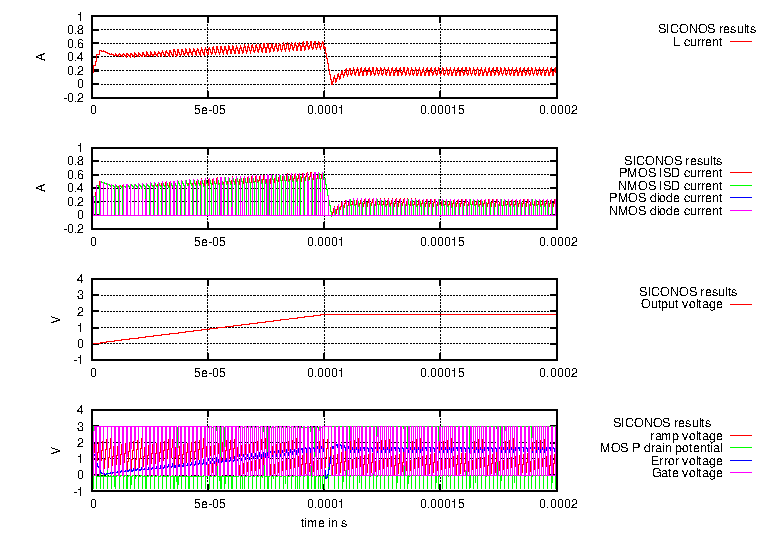
\includegraphics[scale=1.2,angle=0]{simu_siconos_0p2ms_1p0ns.eps}
\end{center}
\caption[SICONOS results, buck \protect\& load resistor (first~$200~\mu s$)]
{SICONOS simulation results, buck converter with a load resistor (first~$200~\mu s$)}
\label{fig-buck-resistor-simu-sico-0p2ms-1p0ns}
\end{figure}

\begin{figure}[hbtp]
\begin{center}
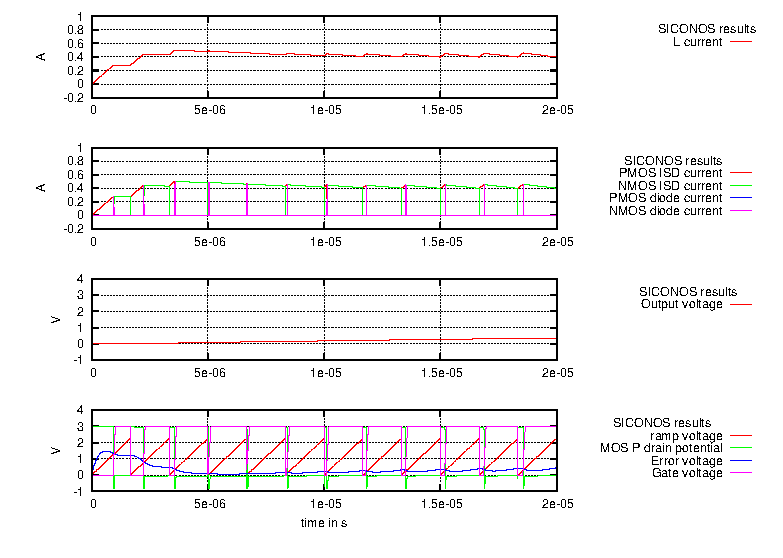
\includegraphics[scale=1.2,angle=0]{simu_siconos_0p02ms_1p0ns.eps}
\end{center}
\caption[SICONOS results, buck \protect\& load resistor (first~$20~\mu s$)]
{SICONOS simulation results, buck converter with a load resistor (first~$20~\mu s$)}
\label{fig-buck-resistor-simu-sico-0p02ms-1p0ns}
\end{figure}

\begin{figure}[hbtp]
\begin{center}
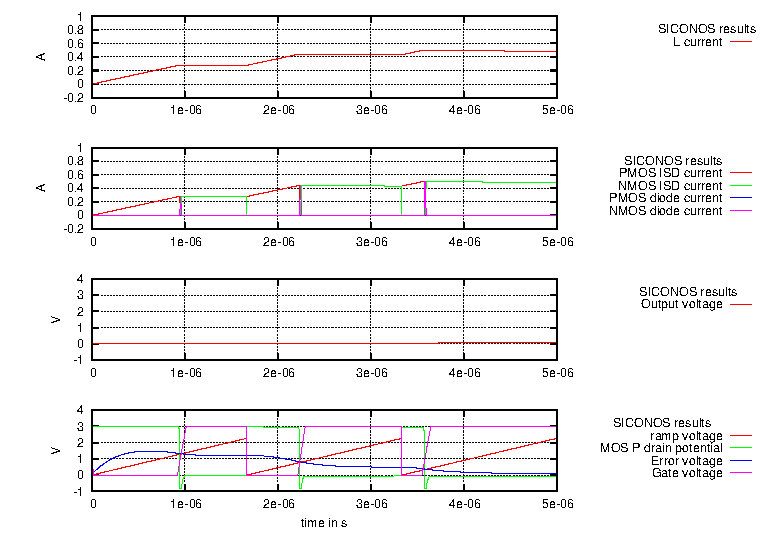
\includegraphics[scale=1.2,angle=0]{simu_siconos_5mics_1p0ns.eps}
\end{center}
\caption[SICONOS results, buck \protect\& load resistor (first~$5~\mu s$)]
{SICONOS simulation results, buck converter with a load resistor (first~$5~\mu s$)}
\label{fig-buck-resistor-simu-sico-5mics-1p0ns}
\end{figure}

\begin{figure}[hbtp]
\begin{center}
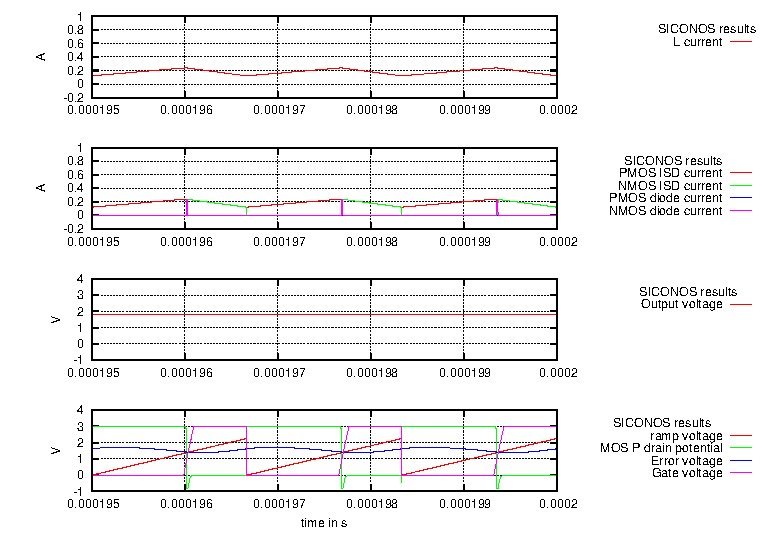
\includegraphics[scale=1.2,angle=0]{simu_siconos_standard.eps}
\end{center}
\caption[SICONOS results, buck \protect\& load resistor , steady state , simple crossings]
{SICONOS simulation results, buck converter with a load resistor\protect\newline
steady state with standard parameters}
\label{fig-buck-resistor-simu-sico-std}
\end{figure}

\begin{figure}[hbtp]
\begin{center}
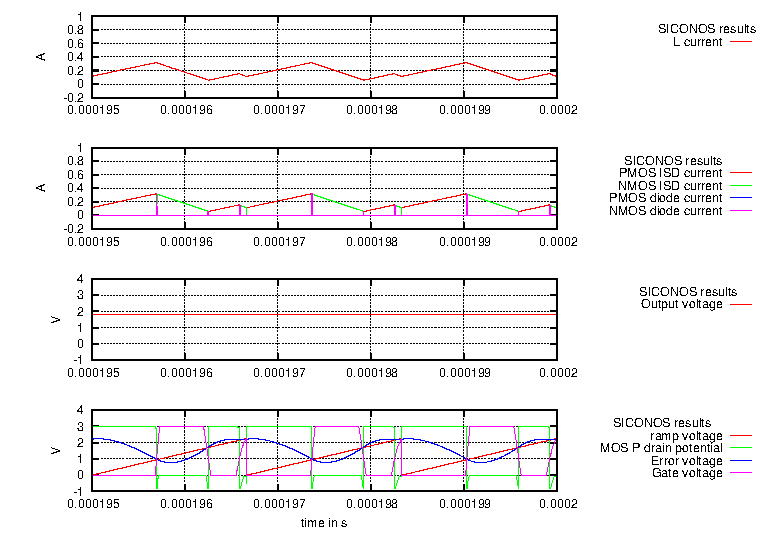
\includegraphics[scale=1.2,angle=0]{simu_siconos_lowLC.eps}
\end{center}
\caption[SICONOS results, buck \protect\& load resistor , steady state , double crossings]
{SICONOS simulation results, buck converter with a load resistor\protect\newline
steady state with $L~=~4~\mu H$, $C~=~10~\mu F$}
\label{fig-buck-resistor-simu-sico-lowLC}
\end{figure}

\begin{figure}[hbtp]
\begin{center}
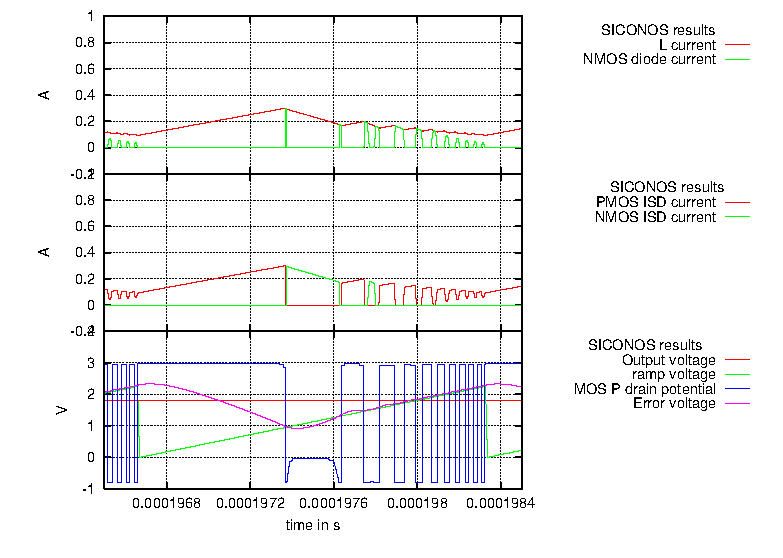
\includegraphics[scale=1.2,angle=0]{simu_siconos_lowLC_badcomp.eps}
\end{center}
\caption[SICONOS results, buck \protect\& load resistor , steady state , sliding mode]
{SICONOS simulation results, buck converter with a load resistor\protect\newline
steady state with $L~=~4~\mu H$, $C~=~10~\mu F$ , $R_{11}~=~10~K\Omega$, $R_{21}~=~8~M\Omega$, $C_{11}~=~10~pF$\protect\newline
exhibiting a sliding mode}
\label{fig-buck-resistor-simu-sico-lowLC-badcomp}
\end{figure}

\begin{figure}[hbtp]
\begin{center}
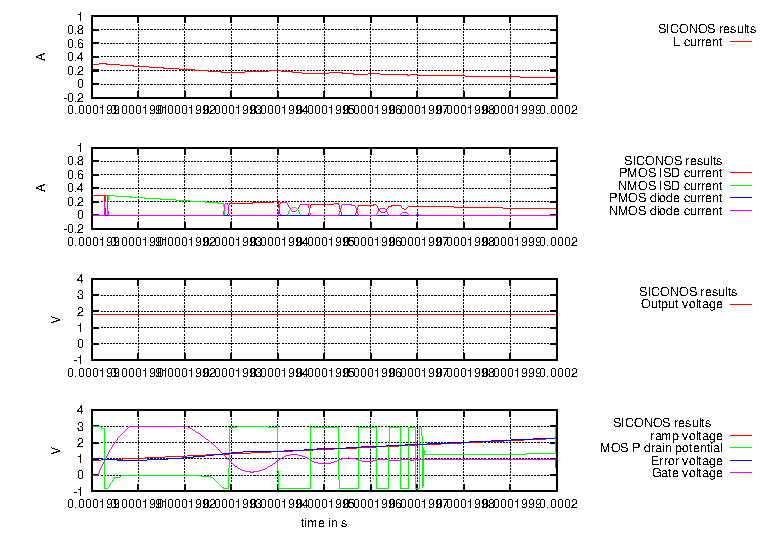
\includegraphics[scale=1.2,angle=0]{simu_siconos_lowLC_badcompzoom.eps}
\end{center}
\caption[SICONOS results, buck \protect\& load resistor , steady state , sliding mode (zoom)]
{SICONOS simulation results, buck converter with a load resistor\protect\newline
steady state with $L~=~4~\mu H$, $C~=~10~\mu F$ , $R_{11}~=~10~K\Omega$, $R_{21}~=~8~M\Omega$, $C_{11}~=~10~pF$\protect\newline
exhibiting a sliding mode (zoom on one ramp)}
\label{fig-buck-resistor-simu-sico-lowLC-badcomp-zoom}
\end{figure}

\begin{figure}[hbtp]
\begin{center}
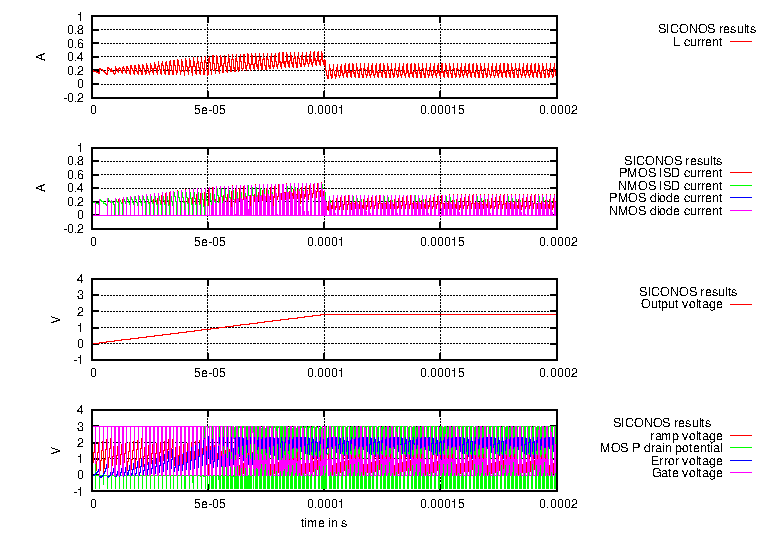
\includegraphics[scale=1.2,angle=0]{simu_siconos_sliding.eps}
\end{center}
\caption[SICONOS results, buck \protect\& load resistor , sliding mode (full simulation)]
{SICONOS simulation results, buck converter with a load resistor\protect\newline
steady state with $L~=~4~\mu H$, $C~=~10~\mu F$ , $R_{11}~=~10~K\Omega$, $R_{21}~=~8~M\Omega$, $C_{11}~=~10~pF$\protect\newline
exhibiting a sliding mode (full $200~\mu s$ simulation)}
\label{fig-buck-resistor-simu-sico-lowLC-badcomp-full}
\end{figure}

\clearpage

\section{Simulation with SPICE : convergence issues related to the MOS model}
The simulation of this circuit was done with several versions of SPICE and two kinds of MOS models :
\begin{itemize}
\item the MOS level 1 model (Schichmann and Hodges model)
\item a simplified model close to 
\end{itemize}

\begin{itemize}
\item Power MOSFETS intrinsic diodes are modelled by the classical Shockley equation with an emission
coefficient $N~=~1$.
\item The comparator is modelled as a non linear voltage controlled voltage source defined as $V_{out}~=~1.5~\cdot~(tanh(10~\cdot~V_{in}) + 1)$.
Thus the 3~segment characteristic used as the non smooth model is regularized to help convergence of SPICE.
\end{itemize}

\begin{description}
\item[with standard values of linear components :] $L~=~10~\mu H$, $C~=~22~\mu F$, $R_{11}~=~15.58~k \Omega$, $R_{12}~=~227.8~k \Omega$, $R_{21}~=~5.613~M \Omega$, $C_{11}~=~20~pF$, $C_{21}~=~1.9~pF$\\
A soft start ($0.1~\mu s$ as rise time) of the power supply $V_I$ was provided to enable the simulation to start. \footnote{This is
not required with the SICONOS algorithms that find a consistent initial solution from scratch.}
It is necessary to release SPICE algorithms tolerance parameters to get a complete simulation. When NGSPICE computes the solution
at one time step with the (iterative) Newton-Raphson algorithm, it validates one iteration if it differs both absolutely and 
relatively from the previous iteration less than given thresholds. The standard threshold values are $1~pA$ for a current, $1 \mu V$ for a 
voltage and $0.001$ for the relative difference. This last parameter was increased up to 0.03 and the time step kept below $0.1~ns$
to enable convergence. It was then possible to complete the simulation in a CPU time of $161$~seconds. Nevertheless, results are impaired
by errors on diode current occurring at switching instants (see figures \ref{fig-buck-resistor-simu-ngspice-0p2ms-std} and
\ref{fig-buck-resistor-simu-ngspice-zoom-std}). Current spikes of more than $10~A$ through the intrinsic NMOS diode are computed. 
NGSPICE checks the convergence only by evaluating the difference between two iterates and does not check if the computed value 
is really a solution of Kirchhoff current law. With a convergence criterion implementing this check, the simulation would likely fail.
\item[with modified values $L~=~4~\mu H$, $C~=~10~\mu F$:] the simulation always fails even with a relative tolerance of~$0.1$ and
a time step of~$10~ps$.
\end{description}

\begin{figure}[hbtp]
\begin{center}
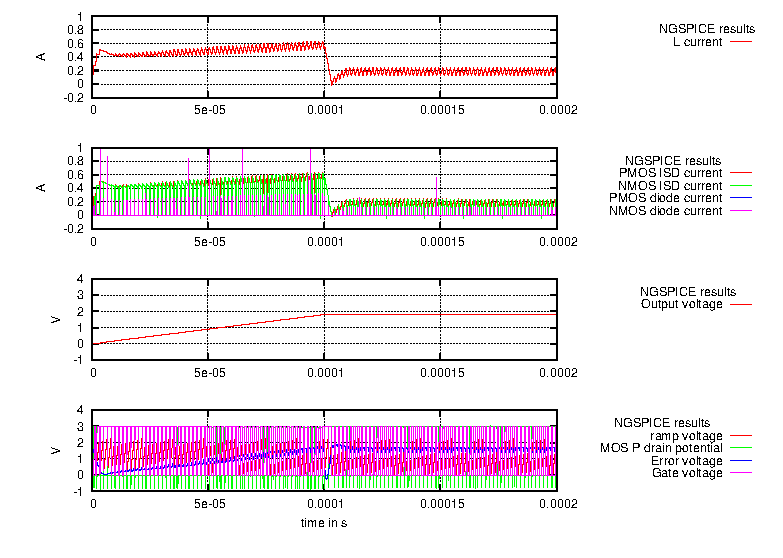
\includegraphics[scale=1.2,angle=0]{simu_ngspice_0p2ms_0p1ns_std.eps}
\end{center}
\caption[NGSPICE results, buck \protect\& load resistor]
{NGSPICE simulation results, buck converter with a load resistor\protect\newline
standard parameters\protect\newline
Erroneous intrinsic NMOS diode current spikes are visible on~the~$2^{nd}$~graph.}
\label{fig-buck-resistor-simu-ngspice-0p2ms-std}
\end{figure}

\begin{figure}[hbtp]
\begin{center}
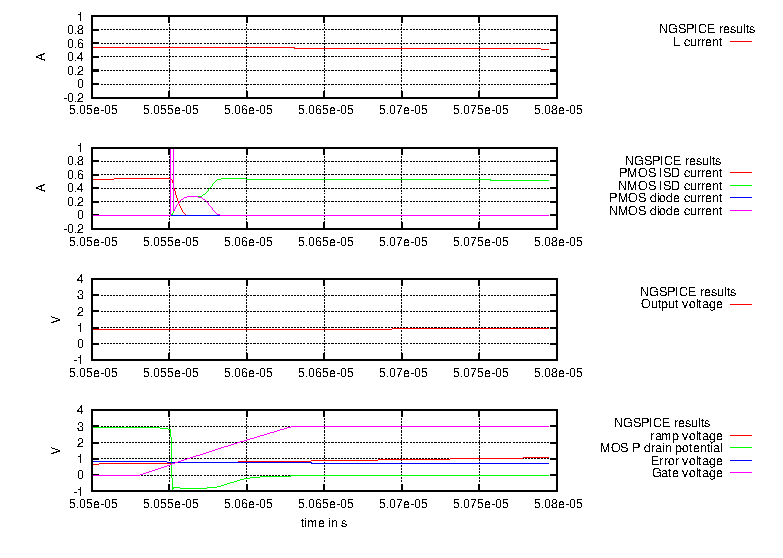
\includegraphics[scale=1.2,angle=0]{simu_ngspice_0p2ms_0p1ns_stdzoom.eps}
\end{center}
\caption[NGSPICE results, buck \protect\& load resistor , zoom]
{NGSPICE simulation results, buck converter with a load resistor\protect\newline
standard parameters, zoom on a NMOS diode current spike}
\label{fig-buck-resistor-simu-ngspice-zoom-std}
\end{figure}

\clearpage

\section{Simulation with PLECS}

PLECS is a Simulink/Matlab toolbox dedicated to the simulation of power electronics circuits.
(see \url{http://www.plexim.com}). The electronic circuits are modelled as hybrid systems:
at each instant, the circuit is described according to one of a set of topologies specified
by the ON or OFF state of ideal switches (diodes, transistors\dots). A topology is
valid when the computed value of some variables (for instance a diode current or voltage) is kept within some
bounds. When a topology is no more valid, a new topology has to be found as well as the possible jump
of variables linked to this topology switching. Even if this approach targets the same kind of systems
as the non-smooth dynamics, its models and algorithms differ mainly in :\\
\\
\begin{tabular}{|p{6cm}|p{6cm}|}
\hline
\textbf{Hybrid systems} & \textbf{Non-smooth dynamical systems} \\
\hline
Each topology is described by a separate set of equations. & 
A single set of equations and constraints describes the whole system. \\
 & \\
Checking the topology switching conditions is critical and may be computationally expensive. &
There is no topology switching : constraints are met at each time step. \\
 & \\
Determining the new topology and the new state value after a topology switch is not obvious.
It may be quick if it can benefit from prior knowledge about the circuit's operation but may also involve heavy computations to check
all possible transitions if no rule is available. &
At each time step, the new values are computed to meet equations and constraints thanks to proper
time integration schemes and one step problem solving based on optimization algorithms \\
\hline
\end{tabular}
\\
\\
The switch models (diodes and transistors) available in the PLECS toolbox are ideal : the transistors
are supposed to be controlled by a boolean signal forcing a conducting or blocking state. 
The power NMOS and PMOS are controlled by opposite signals issued from the feedback loop, thus there is no
flyback conduction by the NMOS diode (see description of the PLECS circuit and the Simulink model in appendix
\ref{modele-PLECS-buckresistor}).

The CPU time required to achieve the simulation of $200~\mu s$ varies between $2~min~15~s$ and $6~min~50~s$ on a 
Pentium~4 clocked at 3~GHz, depending on the values of the resistors, capacitors and inductor. This should be compared
to the $24~s$ of the SICONOS simulation, \textbf{obtained independently from these components values}. This demonstrates
the robustness and efficiency of the time-stepping scheme and the one step solving algorithms of SICONOS.

Figures \ref{fig-buck-resistor-simu-plecs-0p2ms-std} and \ref{fig-buck-resistor-simu-plecs-zoom-std} show the results
when the standard parameters are used : $L~=~10~\mu H$, $C~=~22~\mu F$, $R_{11}~=~15.58~k \Omega$, $R_{12}~=~227.8~k \Omega$,
$R_{21}~=~5.613~M \Omega$, $C_{11}~=~20~pF$, $C_{21}~=~1.9~pF$.

Figures \ref{fig-buck-resistor-simu-plecs-0p2ms-sliding} and \ref{fig-buck-resistor-simu-plecs-zoom-sliding} show the results
when the parameters yielding a sliding mode are used : $L~=~4~\mu H$, $C~=~10~\mu F$, $R_{11}~=~10~k \Omega$, $R_{12}~=~227.8~k \Omega$,
$R_{21}~=~8~M \Omega$, $C_{11}~=~10~pF$, $C_{21}~=~1.9~pF$.

\begin{figure}[hbtp]
\begin{center}
\includegraphics[scale=0.8,angle=270]{simu_plecs_buckresistor_std0p2ms.eps}
\end{center}
\caption[PLECS results, buck \protect\& load resistor , simple crossings]
{PLECS simulation results, buck converter with a load resistor\protect\newline
standard parameters}
\label{fig-buck-resistor-simu-plecs-0p2ms-std}
\end{figure}

\begin{figure}[hbtp]
\begin{center}
\includegraphics[scale=0.8,angle=270]{simu_plecs_buckresistor_stdzoom.eps}
\end{center}
\caption[PLECS results, buck \protect\& load resistor , steady state , simple crossings]
{PLECS simulation results, buck converter with a load resistor\protect\newline
standard parameters (zoom view of steady state)}
\label{fig-buck-resistor-simu-plecs-zoom-std}
\end{figure}

\begin{figure}[hbtp]
\begin{center}
\includegraphics[scale=0.8,angle=270]{simu_plecs_buckresistor_sliding0p2ms.eps}
\end{center}
\caption[PLECS results, buck \protect\& load resistor , sliding mode]
{PLECS simulation results, buck converter with a load resistor\protect\newline
$L~=~4~\mu H$, $C~=~10~\mu F$ , $R_{11}~=~10~K\Omega$, $R_{21}~=~8~M\Omega$, $C_{11}~=~10~pF$\protect\newline
exhibiting a sliding mode}
\label{fig-buck-resistor-simu-plecs-0p2ms-sliding}
\end{figure}

\begin{figure}[hbtp]
\begin{center}
\includegraphics[scale=0.8,angle=270]{simu_plecs_buckresistor_slidingzoom.eps}
\end{center}
\caption[PLECS results, buck \protect\& load resistor , steady state , sliding mode]
{PLECS simulation results, buck converter with a load resistor\protect\newline
$L~=~4~\mu H$, $C~=~10~\mu F$ , $R_{11}~=~10~K\Omega$, $R_{21}~=~8~M\Omega$, $C_{11}~=~10~pF$\protect\newline
exhibiting a sliding mode (zoom view of ``steady'' state)}
\label{fig-buck-resistor-simu-plecs-zoom-sliding}
\end{figure}

\clearpage
\chapter{Test case 2 : a buck converter loaded by a resistor and an inverter chain}
An inverter chain is supplied by the converter in parallel with the resistor. The input of 
this chain starts to oscillate between $0$ and $1.8~V$ after $150~\mu s$, i.e~$50~\mu s$
after the reference voltage reaches $1.8~V$.

The simulated circuit is shown in figure \ref{fig-buck-inverters}.

\begin{figure}[h]
\centerline{
  \scalebox{0.8}{
     \input{buck_inverters.pstex_t}
  }
}
\caption{Buck converter supplying a resistor load and an inverter chain}
\label{fig-buck-inverters}
\end{figure}

\section{Simulation as a non-smooth dynamical system with SICONOS}
The inverter MOSFETs are modelled with a piecewise linear characteristic~$I_{DS}~=~f(V_{GS},V_{DS})$.
Their parameters are:
\begin{description}
\item[Transconductance $KP$:] $4.3\cdot10^{-5}~A.V^{-2}$ for the PMOS , $12.9\cdot10^{-5}~A.V^{-2}$ for the NMOS
\item[Threshold voltage:] $-0.6~V$ for the PMOS and $0.6~V$ for the NMOS
\item[Output capacitive load :] $20~fF$
\end{description}

Two chain lengths were tested :

In the first case, the chain includes only 2 inverters to enable a CPU time comparison with PLECS
whose evaluation version is limited to 6~switches.
To emulate a large current drawn from the output of the converter, the 2 inverters chain
is supposed to be~8000~times large, i.e~8000~chains switching simultaneously as a synchronous
logic circuit. The transconductance and capacitance are therefore multiplied by~8000. The
switching frequency of the chain input is~$200~MHz$.
The CPU time required to achieve the simulation of~$200~\mu s$ with a~$1~ns$ time step 
is~$52$~seconds on a Pentium~4 clocked at 3~GHz.
Results are displayed on figures \ref{fig-buck-inverter-simu-sico1p0ns-std} and 
\ref{fig-buck-inverter-simu-sico1p0ns-stdzoom1}. Figure \ref{fig-buck-inverter-simu-sico0p5ns-stdzoom1}
shows the start-up of the inverters switching simulated with a~$0.5~ns$ time step to enhance
the waveform accuracy.
\\
\begin{figure}[hbtp]
\begin{center}
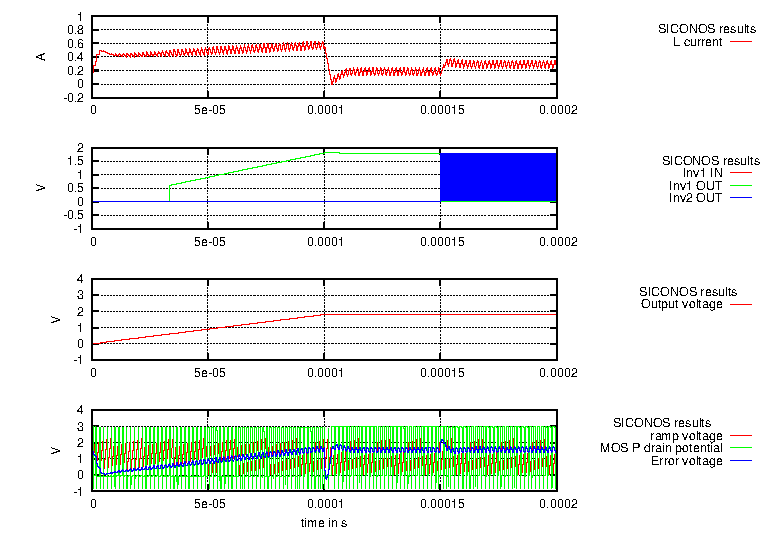
\includegraphics[scale=1.2,angle=0]{simu_sico_buckinv_std1p0ns.eps}
\end{center}
\caption[SICONOS results, buck \protect\& load resistor \protect\& inverters (first~$200~\mu s$)]
{SICONOS simulation results, buck converter supplying a load resistor and an inverter chain (first~$200~\mu s$)}
\label{fig-buck-inverter-simu-sico1p0ns-std}
\end{figure}

\begin{figure}[hbtp]
\begin{center}
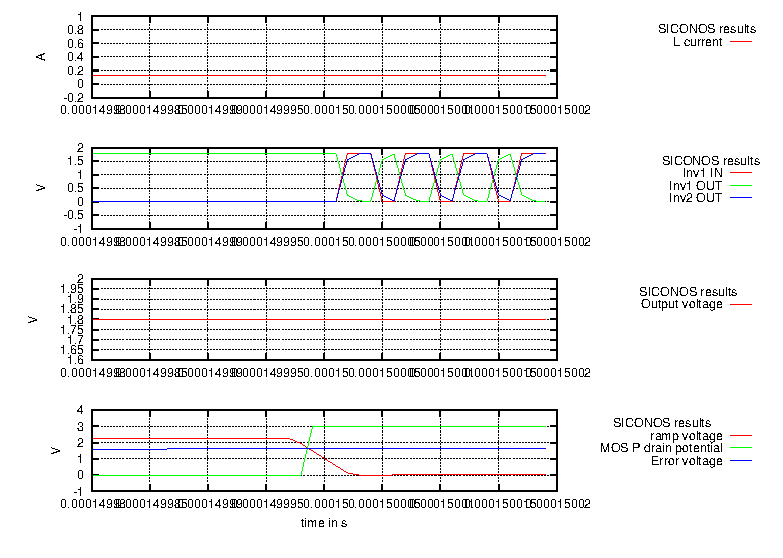
\includegraphics[scale=1.2,angle=0]{simu_sico_buckinv_std1p0nszoom1.eps}
\end{center}
\caption[SICONOS results, buck \protect\& load resistor \protect\& inverters (zoom)]
{SICONOS simulation results, buck converter supplying a load resistor and an inverter chain\protect\newline
Zoom on the start-up of the inverter chain (time~step~=~$1~ns$)}
\label{fig-buck-inverter-simu-sico1p0ns-stdzoom1}
\end{figure}

\begin{figure}[hbtp]
\begin{center}
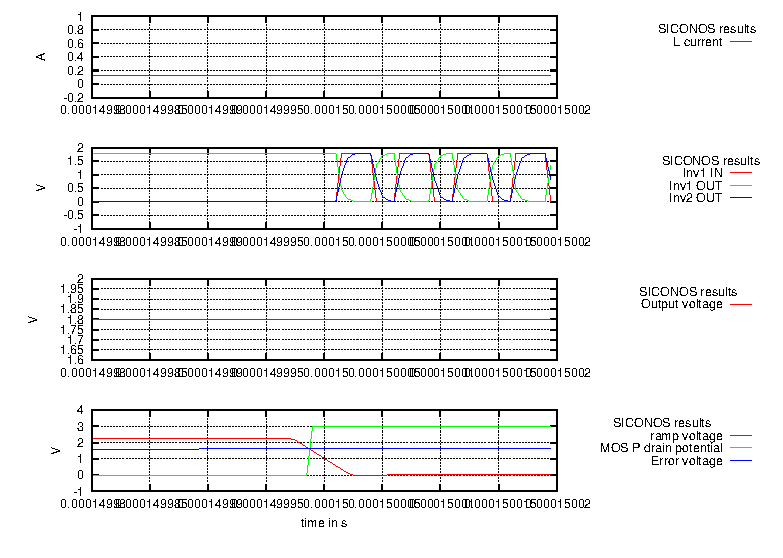
\includegraphics[scale=1.2,angle=0]{simu_sico_buckinv_std0p5nszoom1.eps}
\end{center}
\caption[SICONOS results, buck \protect\& load resistor \protect\& inverters (zoom)]
{SICONOS simulation results, buck converter supplying a load resistor and an inverter chain\protect\newline
Zoom on the start-up of the inverter chain (time~step~=~$0.5~ns$)}
\label{fig-buck-inverter-simu-sico0p5ns-stdzoom1}
\end{figure}

\clearpage
A 100 inverters long chain was also simulated. The reference voltage rises from 0 to~$1.8~V$ in~$50~\mu s$, and the
chain input starts to switch~$30~\mu s$ later at~$25~MHz$. A~$3~\Omega$~load resistor is supplied in parallel
with the inverter chain. To emulate a large current drawn from the output of the converter, the~100~inverters chain
is supposed to be~2400~times large, i.e~2400~chains switching simultaneously as a synchronous
logic circuit. The transconductance and capacitance are therefore multiplied by~2400.

The CPU time required to achieve the simulation of~$100~\mu s$ with a~$0.25~ns$ time step 
is~3~hours on a Pentium~4 clocked at 3~GHz.
Results are displayed on figure \ref{fig-buck-inverter100-simu-sico0p25ns-std}.
\\
\begin{figure}[hbtp]
\begin{center}
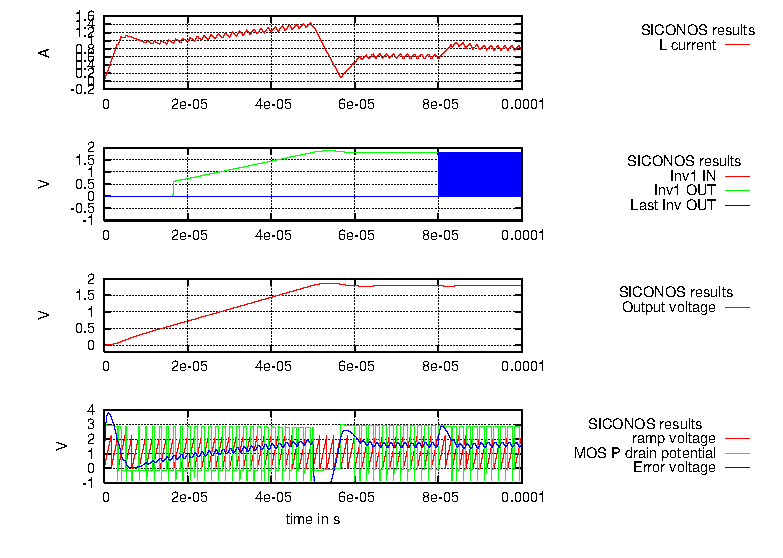
\includegraphics[scale=1.2,angle=0]{simu_sico_buck100inv_std0p25ns.eps}
\end{center}
\caption[SICONOS results, buck \protect\& load resistor \protect\& 100~inverters (first~$100~\mu s$)]
{SICONOS simulation results, buck converter supplying a load resistor and a 100 inverters chain (first~$100~\mu s$)}
\label{fig-buck-inverter100-simu-sico0p25ns-std}
\end{figure}

\clearpage

\section{Simulation with PLECS}
Only 2 inverters could be used due to limitations of the evaluation version.
The inverter MOS transistors are ideal switches with a $R_{ON}$ value of~$0.54~\Omega$ to match
approximately the transconductance of the~8000~parallel MOS modelled in SICONOS. The load capacitor
is set to~$8000~\times~20~fF~=~0.16~nF$ (see description of the PLECS circuit and the Simulink model in appendix
\ref{modele-PLECS-buckinverters}).

The CPU time required to achieve the simulation of~$200~\mu s$ is~$4~hours~8~min$ on a Pentium~4 clocked at 3~GHz,
i.e~300~times the SICONOS simulation time. 

Results are displayed on figures \ref{fig-buck-inverter-simu-plecs-std0p2ms} and 
\ref{fig-buck-inverter-simu-plecs-stdzoom}.

\begin{figure}[hbtp]
\begin{center}
\includegraphics[scale=0.8,angle=270]{simu_plecs_buckinverters_std0p2ms.eps}
\end{center}
\caption[PLECS results, buck \protect\& load resistor \protect\& inverters (first~$200~\mu s$)]
{PLECS simulation results, buck converter supplying a load resistor and an inverter chain (first~$200~\mu s$)}
\label{fig-buck-inverter-simu-plecs-std0p2ms}
\end{figure}

\begin{figure}[hbtp]
\begin{center}
\includegraphics[scale=0.8,angle=270]{simu_plecs_buckinverters_stdzoom.eps}
\end{center}
\caption[PLECS results, buck \protect\& load resistor \protect\& inverters (zoom)]
{PLECS simulation results, buck converter supplying a load resistor and an inverter chain\protect\newline
Zoom on the start-up of the inverter chain}
\label{fig-buck-inverter-simu-plecs-stdzoom}
\end{figure}

\chapter{Conclusion}
A full buck converter supplying both a constant load and a small switching circuit was simulated using
three different classes of algorithms.


The NGSPICE approach whose models are based on regular functions fails to achieve the simulation. Maybe
commercial software packages involve additional tricks to improve convergence, however this remains to be checked.


The PLECS approach enables to simulate a low number of switches in an acceptable time provided that events
are not too frequent. When fast clocked circuitry is added, the simulation time rises high, and it probably happens also
when the number of switches is increased.\footnote{The evaluation version is limited to 6 switches.}


The SICONOS approach allows to perform simulations in reasonable time, and thus to do quickly parametric studies
while keeping the modeling of the main characteristics of components. Furthermore, the algorithms currently implemented
in the platform are initial versions. Future major enhancements will very likely improve the speed without 
impairing accuracy.
\\
The CPU time and convergence results are summarized hereafter :
\newpage

\begin{tabular}{|p{3cm}|p{3cm}|p{3cm}|p{3cm}|}
\hline
 & \textbf{NGSPICE} & \textbf{PLECS} & \textbf{SICONOS} \\
\hline
Buck converter & 161 s or failed & 135 s to 410 s & 24 s \\
load : resistor & {\small erroneous } & {\small very approximate } & {\small slightly approximate }\\
\hline
Buck converter & failed & 4 hours 8 min & 52 s \\
load : resistor \& inverters &   & {\small very approximate } & {\small slightly approximate }\\
\hline
\end{tabular}
\newline
\newline

By ``\textit{very approximate}'', we mean that PLECS models the MOS behavior as fully ideal : it acts as an open or closed
switch controlled by a boolean signal.

By ``\textit{slightly approximate}'', we mean that SICONOS models the MOS behavior electrically with a piecewise
linear characteristic $I_{DS} = f(V_{GS},V_{DS})$.

\appendix

\chapter{PLECS/Simulink model of the buck converter with a load resistor}
\label{modele-PLECS-buckresistor}

\begin{figure}[hbtp]
\begin{center}
\includegraphics[scale=0.8,angle=270]{circuitPLECS.eps}
\end{center}
\caption{PLECS circuit part of the buck converter with a load resistor}
\end{figure}

\begin{figure}[hbtp]
\begin{center}
\includegraphics[scale=0.8,angle=270]{modeleSimulinkBuckResistor.eps}
\end{center}
\caption{Simulink model of the buck converter with a load resistor}
\end{figure}

\chapter{PLECS/Simulink model of the buck converter supplying a resistor and inverters}
\label{modele-PLECS-buckinverters}

\begin{figure}[hbtp]
\begin{center}
\includegraphics[scale=0.8,angle=270]{circuitBuckInvertersPLECS.eps}
\end{center}
\caption{PLECS circuit part of the buck converter supplying a resistor and inverters}
\end{figure}

\begin{figure}[hbtp]
\begin{center}
\includegraphics[scale=0.8,angle=270]{modeleBuckInvertersPLECS.eps}
\end{center}
\caption{Simulink model of the buck converter supplying a resistor and inverters}
\end{figure}

\bibliographystyle{alpha}
\bibliography{biblio}

\listoffigures

\end{document}
